\documentclass[10pt]{article}

\usepackage[T1]{fontenc}
\usepackage[utf8]{inputenc}
\usepackage{lmodern}
\usepackage{microtype}
\usepackage{seqsplit}
\usepackage[margin=0.82in]{geometry}
\usepackage{booktabs}
\usepackage{tabularx}
\usepackage{graphicx}
\usepackage{float}
\usepackage[section]{placeins}
\usepackage{xcolor}
\usepackage{enumitem}
\usepackage[font=small,labelfont=bf]{caption}
\usepackage[round,authoryear]{natbib}
\usepackage{xurl}
\usepackage{hyperref}

\definecolor{evidencegray}{HTML}{666666}
\hypersetup{
  colorlinks=true,
  linkcolor=black,
  citecolor=black,
  urlcolor=blue,
  pdftitle={Deploying Qwen3-1.7B on iPhone with Apple Core AI},
  pdfauthor={Yi Shi and Mengni Wu}
}
\setlist{nosep,leftmargin=*}
\setlength{\parskip}{4pt}
\setlength{\parindent}{0pt}
\DeclareRobustCommand{\evidence}[1]{}
\DeclareRobustCommand{\artifact}[1]{\nolinkurl{#1}}
\DeclareRobustCommand{\digest}[1]{\texttt{\seqsplit{#1}}}
\graphicspath{{generated/figures/}}

\title{Deploying Qwen3-1.7B on iPhone with Apple Core AI:\\
A Static W8 Implementation and Same-Device Profile Evaluation}
\author{
  Yi Shi\\[-1pt]
  \small\href{mailto:massif0601@gmail.com}{\nolinkurl{massif0601@gmail.com}}\\[-1pt]
  \small\href{https://orcid.org/0009-0002-7894-2703}{ORCID: 0009-0002-7894-2703}
  \and
  Mengni Wu\\[-1pt]
  \small\href{mailto:mengninolab@gmail.com}{\nolinkurl{mengninolab@gmail.com}}\\[-1pt]
  \small\href{https://orcid.org/0009-0004-7465-9067}{ORCID: 0009-0004-7465-9067}
}
\date{August 28, 2026}

\begin{document}
\maketitle

\begin{abstract}
Apple's public \artifact{coreai-models} repository contained no Qwen3-1.7B preset at the audited commit.\evidence{CL-01}
We implement a version-pinned static iOS path with per-tensor W8 K-means-palettized transformer projections, a separately INT8-quantized tied embedding, FP16 compute, fixed KV state, a 4,096-token context, and \artifact{h16p} ahead-of-time compilation with Neural Engine-preferred compute.\evidence{CL-03,CL-04,CL-05}
The selected W8 mechanism achieved 0.996598 mean and 0.959625 minimum logit cosine on a frozen holdout, 98.37\% top-1 agreement, and a 0.003167 mean NLL delta relative to frozen uncompressed-reference outputs.\evidence{CL-06,CL-07}
On an iPhone 15 Pro running iOS 27, the historical W8 artifact completed four six-case suites. An Instruments trace recorded 547 MPSGraph program intervals and 547 Apple Neural Engine Prediction intervals, supporting ANE participation in the traced run.\evidence{CL-08,CL-09}
A separate public W8 rebuild also passed a six-case device suite.\evidence{CL-10,CL-22}
We compare this Static-W8 profile with a Dynamic-INT4 profile on the same device using a frozen 300-example CMRC2018 subset.\evidence{CL-11,CL-12}
Static-W8 scored 59.33 EM / 81.70 F1 and Dynamic-INT4 scored 57.67 EM / 81.42 F1; both paired confidence intervals included zero.\evidence{CL-13,CL-14}
Dynamic-INT4 used less storage and peak process memory and decoded faster, while Static-W8 reached the first token sooner and completed the near-4K prefill workload in less time.\evidence{CL-15,CL-16,CL-17,CL-18,CL-19,CL-20}
Because the profiles differ in several coupled design choices, these measurements compare deployable configurations rather than isolated precision or compute-unit effects.
\end{abstract}

\section{Introduction}

Deploying a language model on a phone requires more than compatible weights. Weight representation, KV-cache allocation, graph shape, compilation target, runtime sessions, and memory release jointly determine whether the model can be compiled and used on a physical device.

Qwen3 provides dense and mixture-of-experts language models with unified thinking and non-thinking behavior \citep{yang2025qwen3}. This report concerns the dense Qwen3-1.7B checkpoint at a fixed upstream revision \citep{qwen3ModelRevision}. Both profiles studied here derive from revision \digest{70d244cc86ccca08cf5af4e1e306ecf908b1ad5e} and publish the same tokenizer SHA-256.\evidence{CL-03}

At Apple \artifact{coreai-models} commit \digest{7062017c8e86c6cf4f49b721ddc3494efcdb7c7d}, the Qwen3 support table and model registry listed 0.6B, 4B, and 8B presets but no 1.7B preset.\evidence{CL-01} Apple issue 116 remained an open model request at the August 28 audit \citep{appleQwen3Issue116}.\evidence{CL-01} Pull request 196 proposed macOS and iOS support but closed without merge after its maintainer reported a local iOS regression; the comment did not disclose a root cause \citep{appleQwen3PR196}.\evidence{CL-02}

Community Core AI artifacts already cover dynamic GPU and stateful INT8 routes, with different devices, graph forms, validation methods, and published materials.\evidence{CL-24,CL-25} We study whether Qwen3-1.7B can be added reproducibly to a static iOS authoring path, compiled for \artifact{h16p}, run through \artifact{LanguageModelSession}, and evaluated against a dynamic profile on the same device.

This report makes four contributions:

\begin{enumerate}
  \item A version-pinned Apple-main patch, compression recipe, metadata, focused tests, export instructions, and \artifact{h16p} AOT procedure for an experimental Qwen3-1.7B iOS preset.\evidence{CL-04,CL-05}
  \item Frozen conversion-fidelity results, repeated physical-device suites, validation of the public W8 artifact, and an Instruments trace showing ANE participation.\evidence{CL-06,CL-07,CL-08,CL-09,CL-10}
  \item A same-device evaluation against Dynamic-INT4 with per-example predictions, paired uncertainty estimates, per-run timing records, storage measurements, and process RSS.\evidence{CL-11,CL-12,CL-13,CL-14,CL-15,CL-16,CL-17,CL-18,CL-19}
  \item Public recipes, a source patch, model artifacts, iOS sample applications, recorded hashes, and the deterministic pipeline used to reproduce the reported numbers.\evidence{CL-22,CL-23}
\end{enumerate}

\section{Background and Related Work}

\subsection{Core AI authoring and runtime}

Apple's public \artifact{coreai-models} repository describes export recipes, reusable authoring primitives, and Swift runtime utilities for integrating \artifact{.aimodel} resources with Core AI on macOS and iOS \citep{appleCoreAIModels2026}.\evidence{CL-26} The repository requires version-27 operating systems and Xcode for the audited release and publishes a registry of model presets.\evidence{CL-26} Its public contribution policy at that commit also states that code pull requests are not being accepted at launch, so the patch in this work is presented as a reproducible reference implementation rather than an accepted upstream change.\evidence{CL-26}

Apple has separately documented transformer deployment on the Apple Neural Engine and model palettization \citep{appleANETransformers2022,applePalettization2026}. Those publications provide the general technical context for static-shape and compressed execution. ANE participation in our implementation is supported by the recorded Core AI trace.\evidence{CL-09}

\subsection{Qwen3-1.7B public status}

Table~\ref{tab:public-status} separates Apple's dated registry state, two community artifacts, and the two profiles evaluated in this work. The repository named \artifact{qwen3-1.7b-CoreAI-official} is a community Hugging Face repository, not an Apple publication. At its frozen model-card revision it reports a dynamic INT4 GPU bundle compiled for \artifact{h18p} and measurements on iPhone 17 Pro; those values are not reused as same-device results here \citep{mlboydaisukeCoreAI2026}.\evidence{CL-24} A second community repository publishes a stateful INT8 \artifact{.aimodel}; its reproduction manifest uses the macOS export path, and its numeric accuracy gate is recorded as not run \citep{kevinqzCoreAI2026}.\evidence{CL-25}

\begin{table}[H]
\centering
\small
\setlength{\tabcolsep}{4pt}
\begin{tabularx}{\textwidth}{@{}>{\raggedright\arraybackslash}p{0.17\textwidth}>{\raggedright\arraybackslash}p{0.19\textwidth}>{\raggedright\arraybackslash}X >{\raggedright\arraybackslash}p{0.23\textwidth}@{}}
\toprule
Work & Route & Public evidence & Boundary \\
\midrule
Apple public Qwen3 registry & Official authoring presets & Qwen3-0.6B, 4B, and 8B; no 1.7B preset at the audited commit & Repository state only at commit 7062017c \\
Apple issue 116 / PR 196 & Open request / closed attempt & Issue open; PR closed and unmerged after a reported local iOS regression & No regression root cause, acceptance, or roadmap commitment \\
mlboydaisuke community artifact & Dynamic INT4 / GPU / h18p & iPhone 17 Pro timing and eight model-card questions & Different device, context, and evaluation protocol \\
kevinqz community artifact & Stateful INT8 .aimodel; macOS export manifest & Structural gate passed; numeric gate not run & No disclosed iPhone AOT or paired benchmark \\
This work: W8 profile & Static W8 / fixed KV / ANE-preferred / h16p & Frozen fidelity gate, iPhone 15 Pro suites, and ANE trace participation & One device class; no exclusive-ANE claim \\
This work: INT4 profile & Dynamic INT4 / growing KV / GPU-preferred / h16p & Same-device paired quality, latency, storage, and RSS comparison & Coupled system profile; no isolated causal attribution \\
\bottomrule
\end{tabularx}
\caption{Public Qwen3-1.7B Core AI status audited 2026-08-28. Community model-card claims are contextual, not re-measured results. \evidence{CL-01,CL-02,CL-24,CL-25}}
\label{tab:public-status}
\end{table}


Our evaluation focuses on a static \artifact{h16p} route on A17 Pro and a controlled comparison with a dynamic route on the same device.

\section{System Profiles}

\subsection{Shared source identity}

The W8 and INT4 artifacts originate from \artifact{Qwen/Qwen3-1.7B} revision \digest{70d244cc86ccca08cf5af4e1e306ecf908b1ad5e}; their manifests record tokenizer SHA-256 \digest{aeb13307a71acd8fe81861d94ad54ab689df773318809eed3cbe794b4492dae4}.\evidence{CL-03} Both cap the evaluated context at 4,096 tokens and target the \artifact{h16p} architecture, but most remaining deployment dimensions differ.\evidence{CL-04,CL-11}

\begin{table}[H]
\centering
\small
\setlength{\tabcolsep}{4pt}
\begin{tabularx}{\textwidth}{@{}p{0.21\textwidth}XX@{}}
\toprule
Dimension & Static-W8 & Dynamic-INT4 \\
\midrule
Transformer weights & W8 per-tensor K-means palettization & INT4 block-32 symmetric-with-clipping \\
Embedding & INT8 per-tensor quantization & not separately reported in the artifact summary \\
Compute & FP16 & FP16 \\
KV cache & FP16 fixed-size & FP16 growing/dynamic \\
Graph & static & dynamic \\
Context cap & 4,096 tokens & 4,096 tokens \\
Preferred compute & neural-engine & gpu \\
AOT target & h16p & h16p \\
\bottomrule
\end{tabularx}
\caption{Compared deployment profiles. The rows are coupled system choices, not independently randomized factors. \evidence{CL-03,CL-04,CL-11}}
\label{tab:profiles}
\end{table}


\subsection{Static-W8 profile}

Static-W8 begins from the unquantized upstream checkpoint. The recipe applies per-tensor, eight-bit K-means palettization to 196 transformer projection weights while excluding the embedding modules from that pass. The iOS authoring path quantizes the tied embedding separately to per-tensor INT8.\evidence{CL-04}

The reference patch adds a Qwen3-1.7B model preset and metadata, introduces the locked recipe, marks the preset experimental, adds focused registry and export-contract tests, and extends iOS conversion-matrix coverage.\evidence{CL-05} Against Apple main commit \digest{04a3fd6cfe9bfae9cf05b1f246cf915d930d1c0a}, the patch applied cleanly; 28 focused tests passed, 42 related iOS conversion tests collected without errors, Ruff passed, and the dry-run resolved FP16 compute, the W8 recipe, 4,096 tokens, and enabled embedding quantization.\evidence{CL-05} The full export was not repeated on that later Apple commit because the relevant LLM authoring path was unchanged; compatibility on that commit is therefore claimed only for patch application, tests, lint, and preset resolution.\evidence{CL-05}

The exported \artifact{.aimodel} is compiled with \artifact{coreai-build} for iOS 27, \artifact{h16p}, and Neural Engine-preferred compute. The historical compiled artifact exposes 34 AOT functions across prompt, context, extension, and query buckets.\evidence{CL-04,CL-08} The runtime loads the resource through \artifact{CoreAILanguageModel} and performs generation using \artifact{LanguageModelSession}.\evidence{CL-08}

\begin{figure}[H]
  \centering
  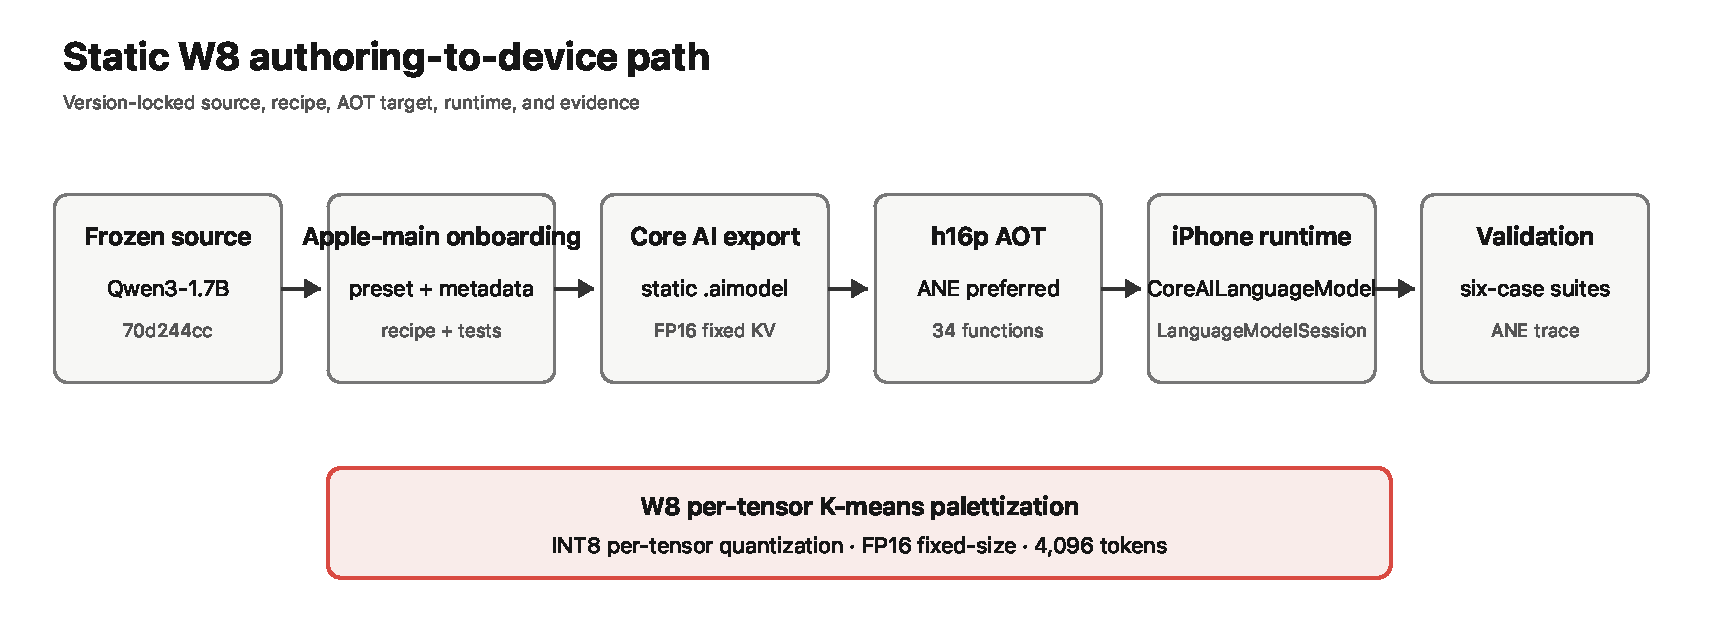
\includegraphics[width=\textwidth]{f1-static-pipeline.pdf}
  \caption{Version-pinned Static-W8 authoring-to-device path. \evidence{CL-04,CL-05,CL-08,CL-09}}
  \label{fig:static-pipeline}
\end{figure}

\subsection{Dynamic-INT4 profile}

Dynamic-INT4 uses block-32 symmetric-with-clipping INT4 transformer weights, FP16 compute, a growing FP16 KV cache, a dynamic graph, and GPU-preferred \artifact{h16p} compilation.\evidence{CL-11} On the test device, the runtime selected the \artifact{coreai-pipelined} engine and reported GPU compute.\evidence{CL-11}

An early pilot relied only on the \artifact{/no_think} prompt suffix. Inspection showed that this did not produce the same template state for both profiles, so the pilot was invalidated and its outputs were excluded. Before the accepted 300-pair run, the runtime was amended to pass \artifact{enable_thinking=false} to the model's chat template; that control was then held constant across both profiles.\evidence{CL-21}

\begin{figure}[H]
  \centering
  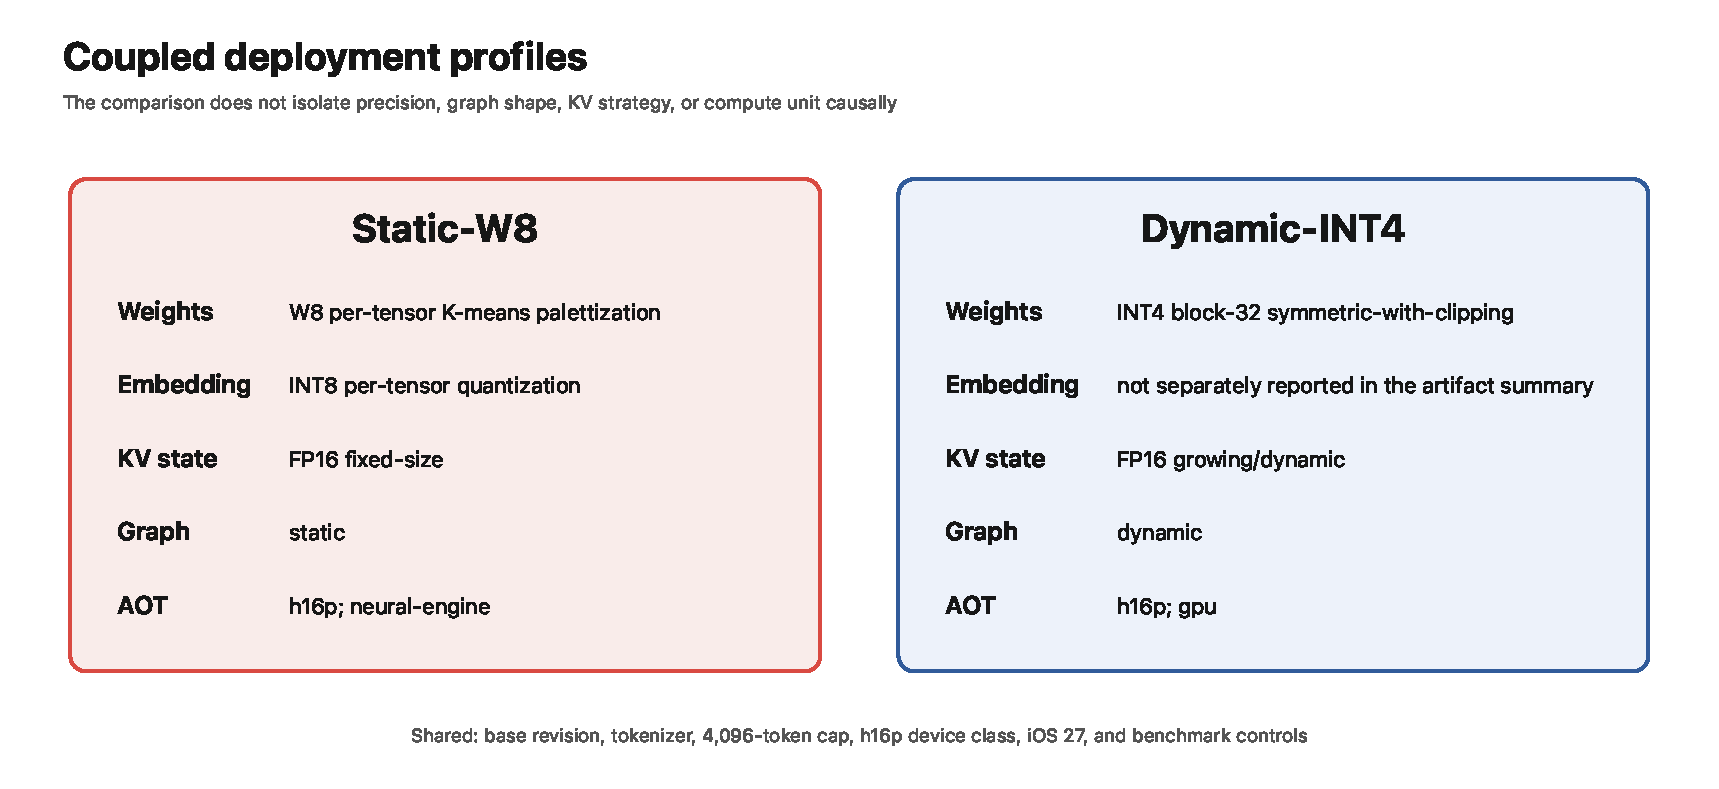
\includegraphics[width=\textwidth]{f2-profile-comparison.pdf}
  \caption{The compared profiles bundle multiple choices. Performance differences cannot be attributed causally to ANE versus GPU or W8 versus INT4 alone. \evidence{CL-04,CL-11,CL-20}}
  \label{fig:profiles}
\end{figure}

\section{Methods}

\subsection{Study design and provenance}

The study protocol was frozen before manuscript drafting. The analysis uses existing public artifacts, predictions, per-run timing records, manifests, and trace summaries. It verifies the inputs listed in \artifact{analysis/source-lock.json}, reconstructs the frozen CMRC sample, reruns deterministic scoring, extracts the accepted timing samples, and generates the quantitative tables and figures. No additional model inference or device measurement is performed by the paper pipeline.

Every admitted artifact is identified by a repository commit or Hub revision and, where applicable, a SHA-256 digest. The current public W8 payload uses the same W8 mechanism but is not byte-identical to the W8 binary used in the historical A/B run. The historical comparison and the public rebuild therefore have separate identity and validation records.\evidence{CL-22}

\subsection{W8 conversion-fidelity selection}

W8 was selected with frozen uncompressed-reference logits and NLL rather than readable-text smoke tests. Uniform W4 and mixed W4/W8 candidates were rejected under the frozen conversion-fidelity contract before the W8 holdout was admitted; representative rejected mean-cosine values ranged from 0.856886 to 0.981232.\evidence{CL-06} The tuning and holdout sets remained separate. These measurements characterize conversion fidelity on the frozen inputs; they are not a downstream task benchmark.\evidence{CL-07}

\subsection{Physical-device validation}

The historical W8 artifact was tested on an iPhone 15 Pro (\artifact{iPhone16,1}, A17 Pro, \artifact{h16p}) running iOS 27. Each six-case suite covered structured output, multi-turn context, an instruction-injection boundary, a 3,790-token long-context retrieval, reasoning output, and unload/reload behavior. Four complete suites ran, and the final suite recorded zero hard failures.\evidence{CL-08}

An Instruments trace was summarized by counts of MPSGraph program and Apple Neural Engine Prediction intervals. The sanitized summary, rather than the original trace bundle, is public. The recorded intervals support ANE participation in the traced inference program.\evidence{CL-09}

The neutral-path public W8 rebuild was then validated separately on the same device class with a six-case suite. This second suite verifies the exact downloadable public payload but is not substituted for the historical A/B binary.\evidence{CL-10,CL-22}

\subsection{Paired CMRC2018 quality comparison}

CMRC2018 is a span-extraction Chinese machine-reading-comprehension dataset \citep{cui2019cmrc}. The paired experiment used a deterministic 300-example subset of its validation split: one question per unique context and 100 examples from each predefined context-length range (276--417, 418--630, and 631--980 characters), interleaved in a fixed order.\evidence{CL-12,CL-27} Equal allocation gives the three length bands equal weight; it does not reproduce the validation split's natural length distribution. The historical protocol records the cut points but no separate statistical derivation for them, so all inferences are limited to this frozen, length-balanced subset. Its SHA-256 is \digest{9fb9d896c96fc2ef0fa9961a5b65d2ac5b8bd09744f717a0a0ecb9f6c9fe05ff}.\evidence{CL-12}

Both profiles used the same tokenizer, chat template with \artifact{enable_thinking=false}, prompt, order, 128-token response budget, temperature zero, and a fresh session per example.\evidence{CL-12} Raw generated text was retained. The paper pipeline rebuilt 3,219 canonical rows from official repository commit \digest{c0eb1b6ba219847457e6af3180da722bbeb656af}, reconstructed the exact frozen sample, and reproduced the published Python-3 scoring JSON byte-for-byte under Python 3.11.15 and NLTK 3.10.0. The original CMRC scorer targeted Python 2; the reproduced result is the explicitly published Python-3 reanalysis.\evidence{CL-12,CL-13}

The primary metrics use the official CMRC mixed Chinese/English EM/F1 procedure. Its \artifact{find_lcs} implementation scores the longest contiguous common token span. The analysis reports paired win/tie counts, 10,000-resample paired bootstrap intervals, and two-sided paired sign tests \citep{efron1979bootstrap}.\evidence{CL-14} Intervals containing zero are reported as inconclusive; no equivalence or non-inferiority test was performed.

The initial feasibility protocol also required Dynamic-INT4 to remain within 1.0 point of Static-W8 on both EM and F1. The observed EM difference was -1.67 points, so this heuristic gate failed. The separately specified paired analysis yielded intervals that included zero.\evidence{CL-13,CL-14}

\subsection{Workload-specific latency and memory}

The speed comparison evaluates complete deployment profiles rather than isolated hardware units. Both variants used the same tokenizer, chat template, prompts, non-thinking control, temperature, and fresh sessions. Each workload had one untimed warm-up followed by three accepted measured samples, with a distinct fixed-width tag to avoid an unreported repeat-input cache.\evidence{CL-17,CL-18,CL-19}

The workloads were: (1) 161 input / 60 output tokens for a compact structured task, (2) 3,790 input / 10 output tokens for near-4K prefill, and (3) 120 input / 256 output tokens for sustained decode.\evidence{CL-17,CL-18,CL-19} One Static-W8 generation terminated after 24 output tokens. Because the sustained-decode statistic was defined for runs reaching at least 200 tokens, this run was recorded, excluded from that statistic, and replaced.\evidence{CL-19} A separate diagnostic pass reused identical prompt tokens and showed cache-sensitive prefill timing; it was excluded before the accepted tagged samples were collected. Sustained-decode throughput is therefore conditional on reaching the protocol's 200-token threshold.

Reported latency values are medians of the three accepted samples, not P95 estimates. Peak RSS means process resident memory observed in the disclosed benchmark, not total system RAM or a universal minimum-memory requirement.\evidence{CL-16,CL-17,CL-18,CL-19}

\section{Results}

\subsection{W8 fidelity and authoring validation}

Table~\ref{tab:w8-fidelity} reports the tuning and frozen-holdout conversion metrics. The holdout mean logit cosine was 0.996598, the minimum was 0.959625, top-1 agreement was 98.37\%, and mean NLL delta was 0.003167.\evidence{CL-07}

\begin{table}[H]
\centering
\small
\setlength{\tabcolsep}{4pt}
\begin{tabular}{@{}lrrrr@{}}
\toprule
Evaluation & Mean cosine & Min. cosine & Top-1 agree. & Mean $\Delta$NLL \\
\midrule
Tuning & 0.997300 & 0.963419 & 98.96\% & 0.004190 \\
Frozen holdout & 0.996897 & 0.953391 & 96.97\% & 0.008880 \\
\bottomrule
\end{tabular}
\caption{W8 authoring-model conversion fidelity relative to the frozen uncompressed reference. Values are case-level macro-averages from the corrected formal fidelity-v2 run, not compiled-device logits or a capability benchmark. \evidence{CL-06,CL-07}}
\label{tab:w8-fidelity}
\end{table}


The later Apple-main compatibility check established patch application, focused tests, related test collection, lint, and preset resolution. It did not repeat the full export on that newer commit and therefore does not claim binary identity with a newly exported payload.\evidence{CL-05}

\subsection{Device execution and trace evidence}

The historical artifact completed four full six-case suites. Its final suite loaded in 11.312 seconds after specialization-cache warm-up, peaked at 2,963.7 MiB process RSS, and returned to 198.7 MiB after unload.\evidence{CL-08} The long-context case consumed 3,790 input tokens, retrieved its tail marker, and produced a first token in 5.627 seconds.\evidence{CL-08}

The trace contained 547 MPSGraph program intervals and 547 Apple Neural Engine Prediction intervals.\evidence{CL-09} The exact public rebuild separately passed all six cases; it peaked at 2,766.4 MiB process RSS and produced the near-4K first token in 5.709 seconds.\evidence{CL-10}

\begin{table}[H]
\centering
\small
\setlength{\tabcolsep}{4pt}
\begin{tabularx}{\textwidth}{@{}p{0.22\textwidth}p{0.22\textwidth}p{0.22\textwidth}X@{}}
\toprule
Evidence object & Measure A & Measure B & Interpretation / identity \\
\midrule
Historical suites & 4 complete & 6 per suite & Pass; zero recorded hard failures \\
Historical final suite & 2,963.7 MiB peak RSS & 198.7 MiB after unload & A-W8-HISTORICAL \\
Historical trace & 547 & 547 & ANE participation; non-exclusive \\
Public rebuild suite & 6 / 6 cases & 2,766.4 MiB peak RSS & A-W8-PUBLIC \\
Public near-4K case & 3,790 input / 10 output & 5.709 s TTFT & Tail marker retrieved \\
\bottomrule
\end{tabularx}
\caption{Physical-device evidence on iPhone 15 Pro / iOS 27. Historical and public W8 payloads use the same mechanism but are not byte-identical. \evidence{CL-08,CL-09,CL-10,CL-22}}
\label{tab:device-evidence}
\end{table}


\subsection{Paired quality}

All 300 examples completed for both profiles without hitting the 128-token budget. W8 produced 178 exact matches (59.33 EM) and 81.70 F1; INT4 produced 173 exact matches (57.67 EM) and 81.42 F1.\evidence{CL-13} The generated responses were byte-identical on 187 of 300 examples.\evidence{CL-13}

The observed Static-W8-minus-Dynamic-INT4 difference was +1.67 EM points with a 95\% bootstrap interval of [-3.00, +6.33] and +0.28 F1 points with an interval of [-2.44, +3.00].\evidence{CL-14} The paired sign-test values were 0.576 for EM and 0.614 for F1.\evidence{CL-14} Both intervals include zero.

\begin{table}[H]
\centering
\small
\setlength{\tabcolsep}{4pt}
\begin{tabular}{@{}lrrrr@{}}
\toprule
Profile & $n$ & EM & F1 & Exact matches \\
\midrule
Static-W8 & 300 & 59.33 & 81.70 & 178 \\
Dynamic-INT4 & 300 & 57.67 & 81.42 & 173 \\
Static-W8 $-$ Dynamic-INT4 & 300 & +1.67 & +0.28 & -- \\
\bottomrule
\end{tabular}
\vspace{3pt}\par\footnotesize W8-minus-INT4 95\% bootstrap intervals: EM [-3.00, +6.33], F1 [-2.44, +3.00]. Sign-test $p$: EM 0.576, F1 0.614.
\caption{Paired CMRC2018 quality on the frozen 300-example subset. Both intervals include zero; no equivalence test was performed. \evidence{CL-12,CL-13,CL-14}}
\label{tab:paired-quality}
\end{table}


\begin{figure}[H]
  \centering
  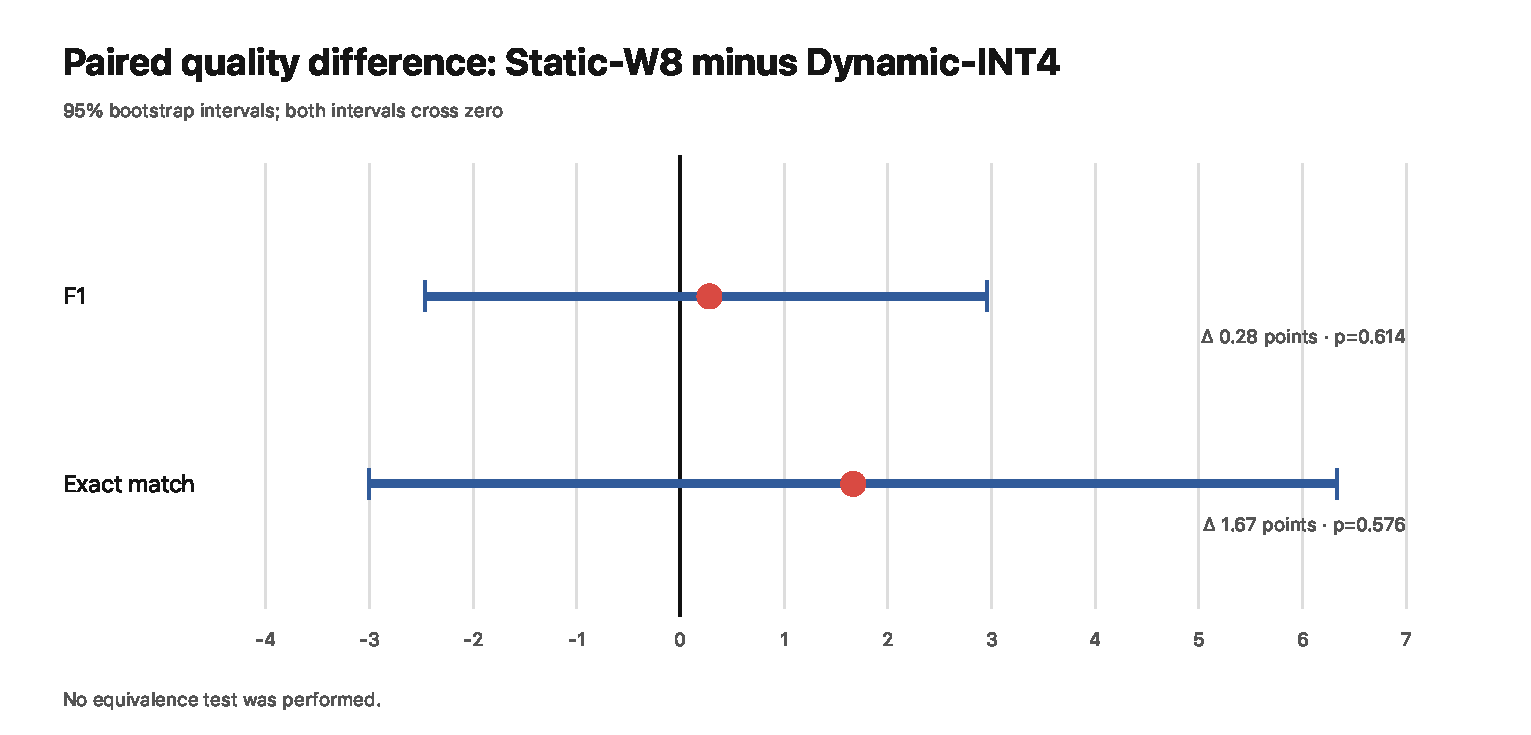
\includegraphics[width=0.88\textwidth]{f3-paired-quality.pdf}
  \caption{Paired Static-W8-minus-Dynamic-INT4 quality differences with 95\% bootstrap intervals. \evidence{CL-13,CL-14}}
  \label{fig:quality}
\end{figure}

\subsection{Storage and process memory}

The historical W8 compiled resource directory occupied 1,714.4 MiB, compared with 924.6 MiB for INT4, a 789.8 MiB (46.1\%) reduction.\evidence{CL-15} Peak process RSS was 2,865.0 MiB for W8 and 1,995.3 MiB for INT4, a reduction of 869.7 MiB (30.4\%) in the disclosed benchmark.\evidence{CL-16}

\begin{table}[H]
\centering
\small
\setlength{\tabcolsep}{4pt}
\begin{tabular}{@{}lrrr@{}}
\toprule
Metric (MiB) & Static-W8 & Dynamic-INT4 & Dynamic-INT4 reduction \\
\midrule
Compiled-model storage & 1,711.4 & 924.6 & 786.8 (46.0\%) \\
Peak process RSS & 3,409.1 & 1,978.0 & 1,431.2 (42.0\%) \\
\bottomrule
\end{tabular}
\caption{Compiled-model storage is the median of four identical estimatedDiskBytes observations converted to MiB; peak process RSS is the maximum after-unload process peak across four physical blocks. \evidence{CL-15,CL-16}}
\label{tab:size-rss}
\end{table}


\subsection{Workload-dependent latency}

For the 161/60 workload, W8 produced the first token in 0.431 seconds versus 1.221 seconds for INT4, but INT4 finished sooner (2.592 versus 3.259 seconds) and decoded faster (43.162 versus 20.505 visible tokens/s).\evidence{CL-17}

For the 3,790/10 workload, Static-W8 reduced TTFT from 13.522 to 5.647 seconds and total time from 13.717 to 6.116 seconds.\evidence{CL-18} Only nine visible decode tokens remained after excluding one reasoning token, so the decode-rate estimate is omitted.

For the 120/256 sustained-decode workload, INT4 reduced total time from 13.292 to 7.159 seconds and increased visible decode from 19.615 to 38.487 tokens/s.\evidence{CL-19} W8 retained the lower median TTFT, 0.404 versus 0.559 seconds.\evidence{CL-19}

\begin{table}[H]
\centering
\small
\setlength{\tabcolsep}{4pt}
\setlength{\tabcolsep}{3pt}
\begin{tabular}{@{}llrrrrr@{}}
\toprule
Input / output & Profile & TTFT$_t$ (s) & TTFT$_v$ (s) & Total (s) & Decode & E2E \\
\midrule
150 / 56 & Static-W8 & 0.242 & 0.242 & 2.234 & 27.542 & 25.066 \\
150 / 22 & Dynamic-INT4 & 1.643 & 1.643 & 2.099 & 45.841 & 10.479 \\
3,778 / 6 & Static-W8 & 3.720 & 3.720 & 3.952 & 21.394 & 1.518 \\
3,778 / 6 & Dynamic-INT4 & 13.393 & 13.393 & 13.522 & 38.556 & 0.444 \\
108 / 256 & Static-W8 & 0.205 & 0.205 & 9.675 & 26.931 & 26.459 \\
108 / 256 & Dynamic-INT4 & 0.390 & 0.390 & 6.454 & 42.210 & 39.760 \\
\bottomrule
\end{tabular}
\caption{Workload medians from 20 completed measurements per profile and workload across four physical blocks. Input and output are median token counts. TTFT$_t$ is token-event TTFT, TTFT$_v$ is visible-token TTFT, and Decode and E2E are visible tokens per second; no P95 is reported. Static-W8 is A-W8-CURRENT at Hub revision \digest{75bbe06906cb5d953e602e3e4fb6364187c81822}. \evidence{CL-17,CL-18,CL-19,CL-20}}
\label{tab:workload-performance}
\end{table}


\begin{figure}[H]
  \centering
  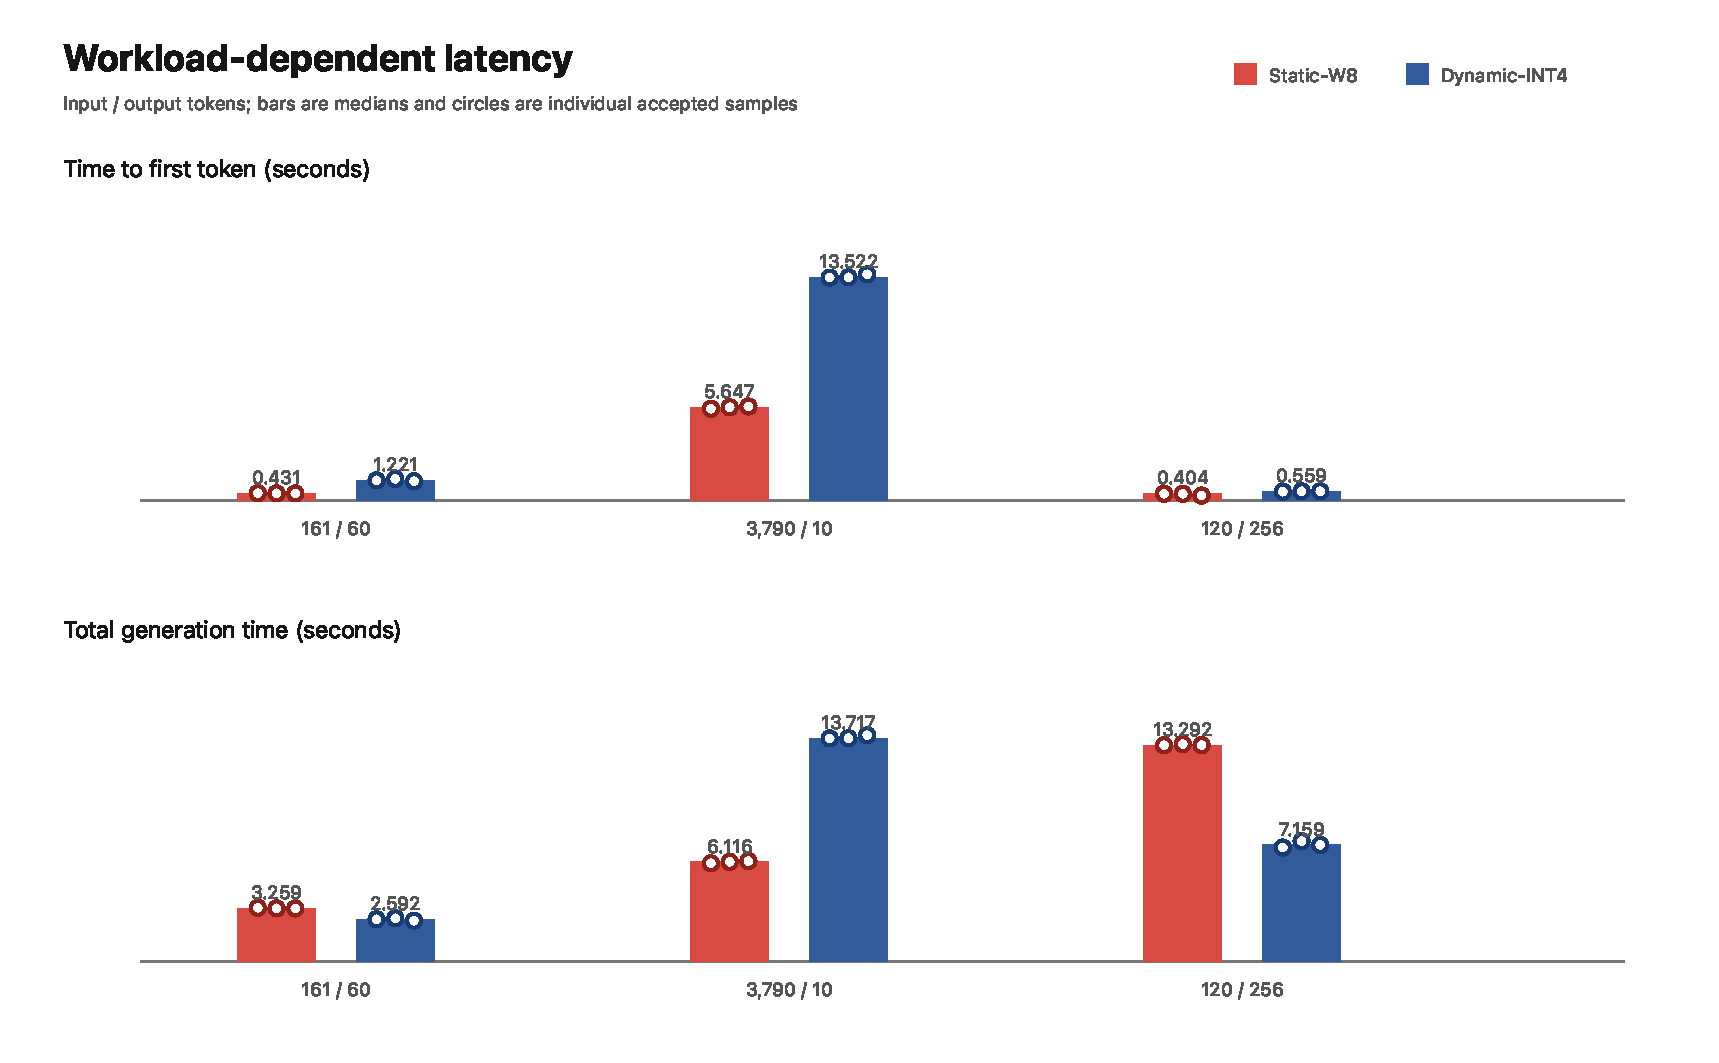
\includegraphics[width=0.90\textwidth]{f4-workload-latency.pdf}
  \caption{TTFT and total generation time for the three workload groups. Bars show medians; circles show the three accepted samples collected after one warm-up. \evidence{CL-17,CL-18,CL-19,CL-20}}
  \label{fig:latency}
\end{figure}

\begin{figure}[H]
  \centering
  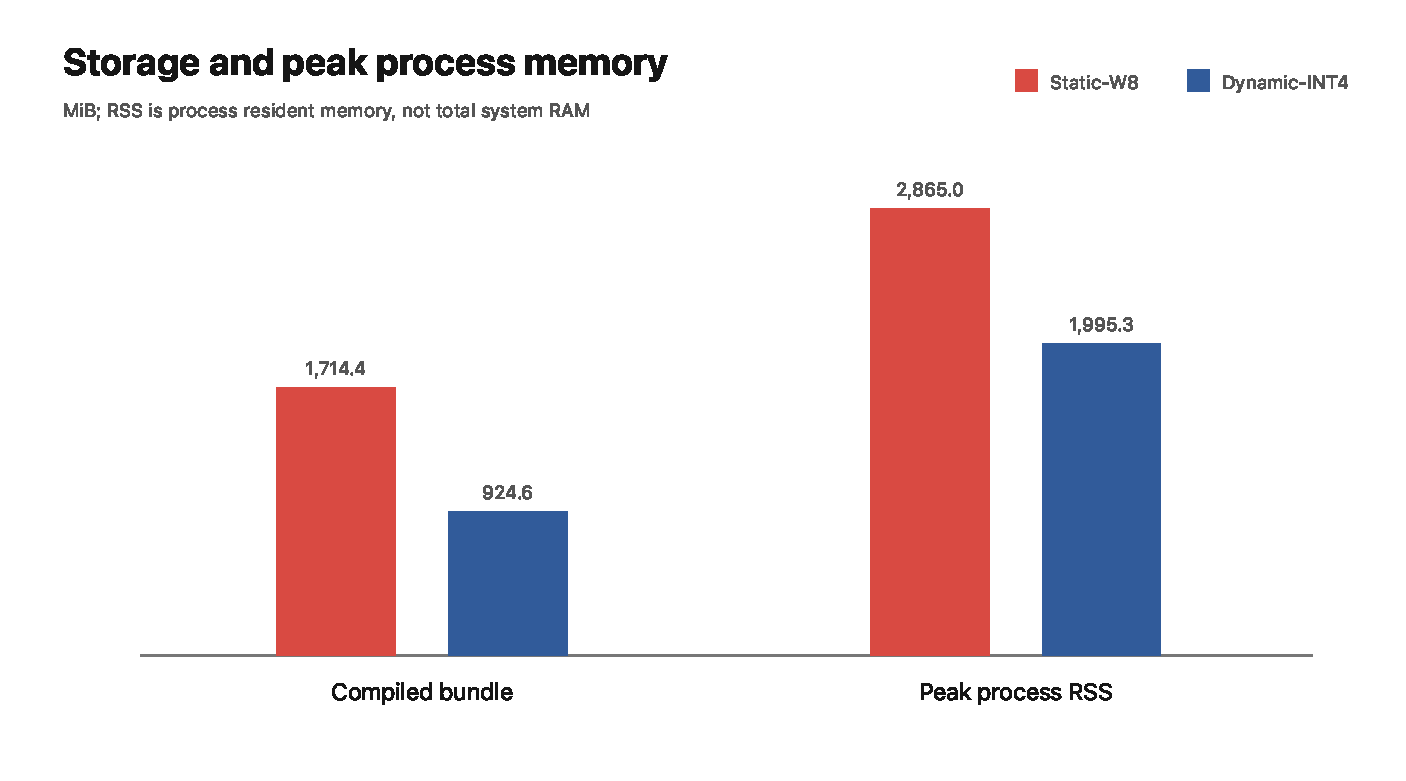
\includegraphics[width=0.82\textwidth]{f5-size-rss.pdf}
  \caption{Compiled bundle size and peak process resident memory. RSS is not total system RAM. \evidence{CL-15,CL-16}}
  \label{fig:size-rss}
\end{figure}

Dynamic-INT4 used less storage and peak RSS and decoded faster in the sustained-generation workload. Static-W8 produced the first token sooner in all three workloads and completed the near-4K workload in less time.\evidence{CL-20}

\section{Discussion}

\subsection{Why the winner changes with workload}

The 161-token structured task combines a modest prefill with enough output for Dynamic-INT4's higher decode rate to overcome its slower first token.\evidence{CL-17} The 3,790-token task reverses the balance: prefill dominates and Static-W8 reaches the first token more than twice as quickly.\evidence{CL-18} The 256-token task places more weight on sustained generation and favors Dynamic-INT4's decode throughput.\evidence{CL-19} The relative performance of the two profiles therefore depends on the balance between prefill and generation in the measured workload.\evidence{CL-20}

Weight precision, embedding treatment, static versus dynamic shape, fixed versus growing KV, engine routing, artifact layout, and memory allocation all change together.\evidence{CL-04,CL-11} The experiment cannot assign the observed differences to any one of these factors.

\subsection{Implications for workload selection}

Dynamic-INT4 performed better on the measured compact-prompt, long-output workload and used less storage and peak process RSS.\evidence{CL-15,CL-16,CL-19} Static-W8 performed better on the measured multi-thousand-token input with a short output.\evidence{CL-18} The two prompt lengths are insufficient to estimate a general crossover point.

CMRC2018 measures extractive Chinese reading comprehension. Transfer to summarization, classification, structured output, instruction boundaries, or bookmark analysis requires task-specific evaluation.\evidence{CL-12,CL-27}

\subsection{Reference implementation}

The published reference implementation includes a tested Qwen3-1.7B preset, the selected compression recipe, an Apple-main patch, \artifact{h16p} compilation instructions, a Swift runtime session, physical-device test records, a sanitized trace summary, and downloadable model artifacts.\evidence{CL-04,CL-05,CL-06,CL-08,CL-09,CL-23} The community GPU and stateful INT8 projects document two other deployment routes.\evidence{CL-24,CL-25}

\section{Reproducibility}

The public W8 repository is frozen at commit \digest{46668db811559ce21b0006f07706a6d0bde08656}; the paired-comparison repository is frozen at \digest{34a4c08a9282bd076b8b5fe154c5507e6a8b3774} \citep{massifW8Repository2026,massifComparison2026}.\evidence{CL-23} W8 empirical evidence is pinned to Hub revision \digest{466ebe2e5cec125fa113ea71503add41bba581a8}. The current model-card revision \digest{be6b5aad19e18bb71be3199eadceb27db7e69724} removes a local device nickname; the model payload and admitted validation file are unchanged. The INT4 Hub citation uses revision \digest{c32b6342c98e5e23363f692e614bccca37f24234}; its predecessor \digest{cb25b3226ee679ee92d0e5af7467d579a6bff66a} is the revision recorded by the original comparison provenance, and the later revision changes documentation while preserving the compiled payload hashes.\citep{massifW8Artifact2026,massifINT4Artifact2026}\evidence{CL-22,CL-23}

The W8 recipe SHA-256 is \digest{dab03ae1dd6c6290a7964e05ebcda7fe027c2bb240174fcf034e64a376be9d72}. The public W8 compiled \artifact{main-h16p.mlirb} SHA-256 is \digest{a7eefeef16708a324f9919890355eb92180ec85eef419ebd5822e8c8afd42f5f}; the INT4 compiled main and \artifact{resources.bin} hashes are \digest{ad953b6bc902accc1f1200a8870012c5dec6b488f0f4ec0f10a9916b16cb56ef} and \digest{37c7f2fcf85625abb32d83ca24e7a9facd33a37f79dbc3afec64d41eb900f8bc}.\evidence{CL-22,CL-23}

The repository separates evidence reconstruction from document compilation. Running \artifact{./analysis/run.sh} fetches the commits and remote objects listed in \artifact{analysis/source-lock.json}, verifies those inputs, reconstructs the CMRC reference sample, recomputes published quality, extracts per-run timing records, and regenerates Tables~\ref{tab:public-status}--\ref{tab:workload-performance} and Figures~\ref{fig:quality}--\ref{fig:size-rss}. It pins Python 3.11.15 and NLTK 3.10.0. Running \artifact{./manuscript/build.sh} then checks the committed generated outputs and compiles the paper with the documented Chrome and Tectonic versions. The reconstructed quality JSON is byte-identical to the published Python-3 result.\evidence{CL-12,CL-13,CL-23}

The dataset text is not redistributed by the paper pipeline. Instead, the official CMRC source commit and SHA-256, canonical-row SHA-256, and frozen-sample SHA-256 are checked before scoring.\evidence{CL-12,CL-27}

The downloadable W8 model is a later rebuild and cannot substitute for the historical A/B binary in an exact replay. The historical predictions, protocols, aggregate results, and recorded hashes remain available, and the public rebuild can be run independently.\evidence{CL-22}

\section{Limitations and Threats to Validity}

\paragraph{Hardware and toolchain.}
All device evidence is from one iPhone 15 Pro / A17 Pro / \artifact{h16p} class running iOS 27 with Xcode 27.0 build \artifact{27A5218g}.\evidence{CL-08,CL-10,CL-11} Other devices and later toolchains were not evaluated.

\paragraph{Coupled profiles.}
The system profiles differ in precision, compression granularity, embedding treatment, graph shape, KV allocation, preferred compute, and artifact layout.\evidence{CL-04,CL-11} The evaluation therefore supports profile-level comparison, not causal attribution to ANE, GPU, W8, or INT4.

\paragraph{Execution trace.}
Only the sanitized trace summary is distributed. It records ANE participation but cannot be used to reconstruct event-level scheduling or exclusive dispatch.\evidence{CL-09}

\paragraph{Quality scope.}
The paired quality run contains a length-balanced subset of 300 CMRC2018 examples rather than the full validation split or its natural length distribution.\evidence{CL-12,CL-13} Confidence intervals include zero, and no equivalence margin was specified.\evidence{CL-14} The initial 1.0-point EM heuristic failed.\evidence{CL-13,CL-14} Complete WikiText-2 perplexity and downstream task evaluations are unavailable.

\paragraph{Timing scope.}
Each workload reports three accepted measured samples after one warm-up, which is insufficient for tail-latency estimates.\evidence{CL-17,CL-18,CL-19} Load observations were cache-sensitive. The sustained-decode comparison is conditional on generation reaching 200 output tokens, and the near-4K case contains too few visible decode tokens for a stable rate estimate.\evidence{CL-18,CL-19}

\paragraph{Energy and lifecycle.}
Energy, battery use, thermal endurance, background execution, and Jetsam behavior were outside the measurement protocol.

\paragraph{Artifact identity.}
The downloadable W8 model uses the same mechanism as the historical A/B model, but it was rebuilt later.\evidence{CL-22} An exact replay still requires the historical binary; the published predictions, protocols, results, and hashes permit inspection of the recorded comparison.

\section{Conclusion}

We implemented a reproducible static Apple Core AI path for Qwen3-1.7B, compiled it for \artifact{h16p}, and ran it through \artifact{LanguageModelSession} on an iPhone 15 Pro with measured ANE participation.\evidence{CL-04,CL-05,CL-08,CL-09,CL-10} Static-W8 retained high conversion fidelity under the frozen inputs. In the same-device evaluation, Dynamic-INT4 used less storage and process memory and decoded faster, whereas Static-W8 reached the first token sooner and completed the long-prompt workload faster.\evidence{CL-07,CL-15,CL-16,CL-17,CL-18,CL-19,CL-20} The released materials allow these workload-dependent trade-offs to be inspected and measured again.

\begingroup
\raggedright
\bibliographystyle{plainnat}
\bibliography{references}
\endgroup

\end{document}
